\documentclass[14pt,a4paper]{article}
\usepackage[utf8]{inputenc}
\usepackage[T1]{fontenc}
\usepackage{amsmath}
\usepackage{color}
\usepackage{amssymb}
\usepackage{makeidx}
\usepackage{graphicx}
\newtheorem{theorem}{Teorema}[section]
\newtheorem{corollary}{Corollario}[section]
\newtheorem{lemma}[theorem]{Lemma}
\newtheorem{prop}[theorem]{Propositione}
\newtheorem{definition}{Definizione}[section]
\newtheorem{observation}[theorem]{Osservazione}
\newtheorem{exemple}[theorem]{Esempio}
%\usepackage{hyperref}
\usepackage{url}
\usepackage{tikz}

\def\cerchio0{(19:4.75cm) circle (0.5cm)}
\def\cerchio1{(21:4.75cm) circle (0.5cm)}
\def\cerchio2{(19:4.75cm) circle (0.5cm)}
\def\secondcircle{(210:1.75cm) circle (2.5cm)}
\def\thirdcircle{(330:1.75cm) circle (2.5cm)}

\title{Crittografia - Appunti su RSA}
\author{Salvatore D'Asta}
\begin{document}
	\maketitle	
	\section{Congruenze modulo p: precisazioni:}
	\subsection{Classi resto modulo n}
	Dati due numeri $ a,b \in \mathbb{Z}=\{insieme\;dei\;numeri\;interi\} $ si dicono congrui modulo $ n\in \mathbb{Z} $:
	\[ a\equiv b \mod n \hspace{1cm}(\textbf{a}\;congruo\;\textbf{b}\;modulo\;\textbf{n})\]
	se $\exists k \in \mathbb{Z}$ tale che $ a=b+k\cdot n $ con $ k \in \mathbb{Z} $
	La congruenza modulo n è una relazione di equivalenza\footnote{\url{https://it.wikipedia.org/wiki/Relazione_di_equivalenza}}
	che \textit{partiziona} l'insieme $ \mathbb{Z} $ creando l'insieme quoziente:
	\[ \mathbb{Z}_n=\{\bar{0},\bar{1},\bar{2},\cdots,\overline{(n-1)}\} \]
	dove l'elemento $ \overline{t}\in \mathbb{Z}_n $ rappresenta tutti i $ k \in \mathbb{Z} $ per i quali vale $ k\equiv t \mod n $
	Nella pratica per trovare a quale classe appartiene il numero $ s\in \mathbb{Z} $ basta calcolare il resto della divisione intera: $ s=k\cdot n+r $ in tal caso $ s\in \bar{r} $
	\\In $ \mathbb{Z}_n $ possiamo definire le stesse operazioni definite in $ \mathbb{Z} $\\
	A titolo d'esempio prendiamo l'elevazione a potenza in $ \mathbb{Z}_7=\{\bar{0},\bar{1},\bar{2},\bar{3},\bar{4},\bar{5},\bar{6}\} $
	\[ \overline{3^2}\equiv \bar{2} \mod7  \]
	infatti $ 3^2=9=7\cdot 1+\boxed{\textbf{2}} $ .\\
	Per convenzione come rappresentante di una classe resto modulo n si prende il più piccolo dei suoi elementi maggiore di zero.
	\subsubsection*{Esempio $ \mathbb{Z}_5=\{\bar{0},\bar{1},\bar{2},\bar{3},\bar{4}\} $:}
	
	
	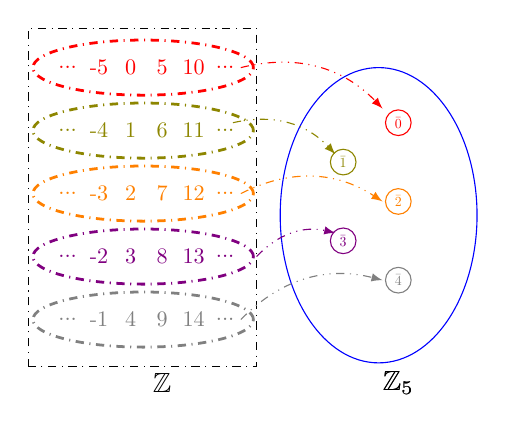
\begin{tikzpicture}
		%\draw [help lines] (0,0) grid (3,2);
		\node [draw, circle,red,scale=.5] at (3,3.8) {$\bar{0}$};
		\node [draw, circle, olive,scale=.5] at (2.3,3.3) {$\bar{1}$};
		\node [draw, circle,orange,scale=.5] at (3,2.8) {$\bar{2}$};
		\node [draw, circle,violet,scale=.5] at (2.3,2.3) {$\bar{3}$};
		\node [draw, circle,gray,scale=.5] at (3,1.8) {$\bar{4}$};
		\draw[dash dot] (-1.7,.7) rectangle (1.2,5);
		\node at (0,0.5) {$ \mathbb{Z} $};
		\draw [yscale=1.5, blue,scale=.5] (5.5,3.5) circle (2.5);
		
		\node at (3,0.5) {$ \mathbb{Z}_5 $};
		\node [red,scale=0.8] at (-0.4,4.5) {0};
		\node [red,scale=0.8] at (0.0,4.5) {5};
		\node [red,scale=0.8] at (0.4,4.5) {10};
		\node [red,scale=0.8] at (-0.8,4.5) {-5};
		\node [red,scale=0.8] at (-1.2,4.5) {...};
		\node [red,scale=0.8] at (0.8,4.5) {...};	
		
		\draw [-latex, bend left,red,dash dot dot] (1,4.5) to (2.8,3.98);
		\node at (3,0.5) {$ \mathbb{Z}_5 $};
		\node [olive,scale=0.8] at (-0.4,3.7) {1};
		\node [olive,scale=0.8] at (0.0,3.7) {6};
		\node [olive,scale=0.8] at (0.4,3.7) {11};
		\node [olive,scale=0.8] at (-0.8,3.7) {-4};
		\node [olive,scale=0.8] at (-1.2,3.7) {...};
		\node [olive,scale=0.8] at (0.8,3.7) {...};	
		%
		\draw [-latex, bend left,olive,dotted,dash dot dot ] (0.9,3.8) to (2.2,3.4); 
		
		\draw [-latex, bend left,orange,dotted,dash dot dot ] (1,2.9) to (2.8,2.8);
		 \node [orange,scale=0.8] at (-0.4,2.9) {2};
		 \node [orange,scale=0.8] at (0.0,2.9) {7};
		 \node [orange,scale=0.8] at (0.4,2.9) {12};
		 \node [orange,scale=0.8] at (-0.8,2.9) {-3};
		 \node [orange,scale=0.8] at (-1.2,2.9) {...};
		 \node [orange,scale=0.8] at (0.8,2.9) {...};
		 
		\draw [-latex, bend left,violet,dotted,dash dot dot ] (1.2,2.1) to (2.2,2.4);
		\node [violet,scale=0.8] at (-0.4,2.1) {3};
		\node [violet,scale=0.8] at (0.0,2.1) {8};
		\node [violet,scale=0.8] at (0.4,2.1) {13};
		\node [violet,scale=0.8] at (-0.8,2.1) {-2};
		\node [violet,scale=0.8] at (-1.2,2.1) {...};
		\node [violet,scale=0.8] at (0.8,2.1) {...}; 
		
		\draw [-latex, bend left,gray,dotted,dash dot dot ] (1,1.3) to (2.8,1.8);
		\node [gray,scale=0.8] at (-0.4,1.3) {4};
		\node [gray,scale=0.8] at (0.0,1.3) {9};
		\node [gray,scale=0.8] at (0.4,1.3) {14};
		\node [gray,scale=0.8] at (-0.8,1.3) {-1};
		\node [gray,scale=0.8] at (-1.2,1.3) {...};
		\node [gray,scale=0.8] at (0.8,1.3) {...}; 	
		
		
		\draw[xscale=4,red,dash dot ,line width=1pt]  (-0.06,4.5) circle(0.35);
		\draw[xscale=4,olive,dash dot ,line width=1pt]  (-0.06,3.7) circle(0.35);
		\draw[xscale=4,orange,dash dot ,line width=1pt]  (-0.06,2.9) circle(0.35);
		\draw[xscale=4,violet,dash dot ,line width=1pt]  (-0.06,2.1) circle(0.35);
		\draw[xscale=4,gray,dash dot ,line width=1pt]  (-0.06,1.3) circle(0.35);			
	\end{tikzpicture}
	
	\subsection{Strutture Algebriche:  gruppi, anelli e campi.}
	Dato un insieme $ A$ e un'operazione $ + $ definita in $ A\times A\longmapsto A $ in modo tale che $ \forall a,b \in A $ sia $ a + b=c \in A $ un operazione che ha questa proprietà viene detta \textit{legge di composizione interna} in $ A $.\\
	\begin{definition}[gruppo]
		Un insieme $ (A,+) $ dotato di legge di composizione interna $ + $ da $ A\times A\longrightarrow A $   è un \textbf{gruppo} abeliano se:
		\begin{itemize}
			\item $ \forall a,b,c\in A \hspace{1cm} (a + b)+ c=a + (b  + c) $ (associativa)
			\item  $\exists e \in A $ tale che  $ \forall a \in A \hspace{1cm} a  + e=e  + a=a$ (elemento neutro)
			\item $ \forall a \in A \hspace{1cm} \exists a^{-1}$ tale che $ a + a^{-1} = a^{-1} + a=e$ (esistenza del reciproco) 
			\item $\forall a,b \in A \hspace{0.5 cm} a+b=b+a $ ( commutativa)
		\end{itemize}
	\end{definition}
	
	 \begin{definition}[anello]
	 	Se $ (A,+) $ è un gruppo abeliano e se è definita una operazione $ \cdot $ da $ A\times A\longrightarrow A $ per la quale valgano le seguenti leggi distributive:
	 	\[ \forall a,b,c \in A \hspace{.5cm}(a+b)\cdot c=a\cdot c+ b\cdot c \hspace{.5cm} (a\cdot b)+c=(a+c)\cdot (b+c)\] allora $ (A,+,\cdot) $ è un \textbf{anello} 
	 \end{definition}
	\begin{definition}[campo]
		Sia $ (A,+,\cdot) $ un \textbf{anello} e sia $ A^*=A-\{0\} $. Se $ (A^*,\cdot) $   è un gruppo abeliano allora è anche un \textbf{campo}\\
		\fbox{Quindi un \textbf{campo} è un anello nel quale $ A^* $ con l'operazione $ \cdot $  è un gruppo abeliano} 
	\end{definition}
	\subsection{L'algoritmo RSA}
	Alice vuole consentire a Bob di inviarle un messaggio $ M $ segreto.
	\begin{enumerate}
		\item 
		\begin{itemize}
			\item Sceglie due numeri primi $ p $ e $ q $ e calcola $ N=p\times q $. (scelti in modo che $ M<N $ )
			\item Calcola $ \varphi(N)=(p-1)\times (q-1) $. 
			\item Trova $ 0<e<\phi(N) $ in modo che $ MCD(e,\varphi(N))=1 $ (cioè siano coprimi).\\ La coppia $ \boxed{(e,N)} $ costituisce la chiave pubblica e viene inviata a Bob.
			\item Alice poi crea la sua chiave privata $ \boxed{(d,N)} $ trovando $d $ tale che \\$ \boxed{e\times d\equiv 1 \mod \varphi(N) } $.
		\end{itemize}
		\item Bob ricevuto $ (e,N) $ calcola: \[ M^e \mod N=C \] e lo invia a Alice. Quest'ultima per decifrare il messaggio eseguirà:\[ C^d \mod N =M \]
	\end{enumerate}
	\subsubsection{Perchè RSA funziona?}
	Ciò accade perchè:
	\begin{equation}\label{key}
		C^d \mod N = M^{e\cdot d} \mod N=M \mod N
	\end{equation}
	e ciò è vero perché avendo scelto $ e $ e $ d $ in modo che $ e\cdot d=k\cdot \phi(N)+1 $ allora posso riscrivere la \eqref{key} in questo modo:
	\begin{equation}\label{E}
		M^{e\cdot d} \mod N=M^{k\cdot \phi(N)+1} \mod N=M^{k\cdot \phi(N)}\cdot M^1 \mod N
	\end{equation}
	per ottenere la tesi è necessario che nella  \eqref{E} valga $ M^{ \phi(N)}=1 $ in $ \mathbb{Z}_N $.
	\\Il teorema di \textbf{Eulero-Fermat} afferma proprio quanto richiesto:\\
	\begin{theorem}[Eulero-Fermat]
		Se M è coprimo con N (cioè $ MCD(M,N)=1 $) allora:
	
		
	\begin{equation}\label{eulero}
		\boxed{M^{\phi(N)} \equiv 1 \mod N}
	\end{equation}
\end{theorem}
	Essendo $ M<N $ allora $ MCD(M,N)=1 $ e quindi soddisfa le ipotesi del teorema.
	\footnote{Il teorema di \textbf{EULERO-Fermat} prevede che se N è coprimo con M allora vale la \ref{eulero} \\Il piccolo teorema di Fermat afferma che se $ p $ è un numero primo allora $ t^p \equiv t  \mod p $ da cui si ottiene, dividendo entrambi i membri per $ t $,  \begin{equation}
			t^{p-1}\equiv 1 \mod p \label{toziente}
		\end{equation} ma la funzione \textbf{toziente di Eulero} $ \phi(p)=\{numero\;di\;valori\;minori\;di\;p\;che\;non\;sono\;divisori\;di\;n\} $  essendo $ p  $  primo sarà $ \phi(p)=(p-1) $ e sostituendo nella \eqref{toziente} ottengo \begin{equation}
			t^{\phi(p)} \equiv 1 \mod p
	\end{equation}}
	\subsubsection{Perchè RSA è sicuro?}
	Per poter decifrare un messaggio ($ C=M^e \mod N $) bisogna disporre della  chiave privata $ d $ ($ M=C^d \mod N $) ma per ricavare la chiave privata $ d $ bisogna conoscere $ \phi(N)=(p-1)\cdot (q-1) $ che equivale a trovare i fattori  $ p $ e $ q $  che generano $ N $. Per i numeri $ N $ molto grandi (rappresentabili con centinaia di cifre), non sono stati ancora trovati  degli algoritmi che ne consentano la fattorizzazione in tempi accettabili.\\ Esistono diversi algoritmi di fattorizzazione, il più semplice consiste nel provare a dividere il numero per tutti i numeri $ n \in \mathbb{Z}$ con $ 1<n<\sqrt{N} $. Questo metodo per numeri molto grandi non risulta efficiente dato che, nel caso pessimo, si potrebbe essere costretti ad effettuare $ \sqrt(N) $ operazioni. In questo caso si dice che l'algoritmo ha complessità $ O\sqrt{N} $ (ordine di radice di N). \\
	Un altro algoritmo, la fattorizzazione di Fermat, sfrutta l'idea che se $ N $ è un numero dispari ed è ottenuto come prodotto di due numeri $ p $ e $ q $,  anch'essi dispari, allora si possono trovare due interi $ a $ e $ b $ tali che:\[ N=(a-b)(a+b) \] 
	Questo perché:\[ N=p q=\left(\frac{p-q}{2}\right)  ^2-\left( \frac{p+q}{2}\right) ^2 \] 
	Infatti:\[ \left(\frac{p-q}{2}\right)  ^2-\left( \frac{p+q}{2}\right) ^2=\frac{1}{4}(p^2+2pq+q^2)-\frac{1}{4}(p^2-2pq+q^2)=pq \]
	Quindi posto:
	\[ \left(\frac{p-q}{2}\right)=a \]
	e
	\[ \left( \frac{p+q}{2}\right)=b \]
	ottengo che $ N=a^2-b^2=(a+b)(a-b) $. \textit{(Si asservi che $ p-q $ e $ p+q $ sono numeri pari perché la somma e la differenza di due numeri dispari dà un numero pari, questo ci assicura che $ a $ e $ b $ sono interi)}.\\ 
	Il problema di trovare i fattori di $ N $ si può ricondurre a trovare $ a $ per il quale si abbia:\[ a^2-N=b^2 \] 
	La ricerca dei fattori consiste nel trovare $ \sqrt{N}<a<N $ in modo che $ a^2-N $ sia intero.
	\subsection{Come calcolare l'esponente privato $ d $ noti $ \phi(N) $ ed $ e $}
	\subsubsection{Metodo di Eulero esteso}
	Indicando con l'operatore $ div $ la  parte intera della divisione  tra due interi ad esempio $ 5\; div\; 2 =2$  e indicando con $ \mod $ l'operatore modulo che fornisce il resto della divisione tra due interi ad esempio $ 5 \mod 2 =1 $
	
	\begin{tabular}{c|c|c}
		$ \phi(N) $	& 0 {\color{red}(a)}&  \\
		\hline
		e	& 1 {\color{red}(b)}&  $ \phi(N)\;div\; e$ {\color{red}(c)}\\
		\hline
		$ \phi(N) \mod e $	& $ {\color{red}a}-{\color{red}b} \cdot {\color{red}c}$ &  \\
		\hline
		&  &  \\
	\end{tabular}
	\\Ad esempio siano $ p=37, q=43 $ allora $ N=37\cdot 43=1591 $ e $ \phi(N)=36\cdot 42=1512  $ e scegliamo $ e=23 $ calcoliamo $ d  $ con l'algoritmo precedente:\\
	\begin{tabular}{c|c|c}
		1512	& 0 &  \\
		\hline
		23	& 1 & 65 \\
		\hline
		17	& -65 & 1 \\
		\hline
		6	& 66 &  2\\
		\hline
		5	& -197 & 1 \\
		\hline
		{\color{blue}1}	& $ {\color{red}263} $ &  \\
	\end{tabular}
	\\ ed infatti posto $ M=24 $ ottengo $ C=M^e \mod N=24^{23} \mod 1591= 146$ ed elevando $ C $ per $ d $ ottengo $ C^d \mod N=146^{263} \mod 1591=24 $
	
	\begin{tabular}{|c|c|c|c|c|}
		\hline
		Indice&Quoziente  &resto  & x & y \\
		\hline
		&  & 20 & 1 & 0 \\
		\hline
		&  & 7 & 0 & 1 \\
		\hline
		&$ 20//7=2 $  & 6 &  &  \\
		\hline
		&  &  &  &  \\
		\hline
		&  &  &  &  \\
		\hline
	\end{tabular}
	
	\section{Dimostrazione del teorema di Eulero-Fermat}
	\subsection{Prima parte - I coefficenti binomiali}
	Il \textbf{coefficiente binomiale} è definito come:\begin{equation*} \binom{p}{i}=\frac{p!}{i!(p-i)!} \hspace{1cm} \forall p,i \in \mathbb{N}  \hspace{0.5cm}  i \leq p \end{equation*}
	e $ \forall n \in \mathbb{N} \hspace{0.5cm} n!=n\cdot (n-1)\cdot (n-2) \cdots 1$\\
	possiamo usare il coefficiente binomiale per calcolare la potenza \hspace{0.5cm}di un binomio:
	\begin{equation*} (A+B)^{p}=\sum_{i=0}^{p} \binom{p}{i}A^{(p-i)}B^i \end{equation*}
	quindi ad esempio:
	\begin{equation*}
		(A+B)^3=\binom{3}{0}A^3B^0+\binom{3}{1}A^2B^1+\binom{3}{2}A^1B^2+\binom{3}{3}A^0B^3= 
	\end{equation*}
	\begin{equation*}
		=A^3+3A^2B+3AB^2+B^3  
	\end{equation*}
	
	Tutto questo vale se si sta operando nell'insieme degli interi, cioè in $ \mathbb{Z }$,
	se invece operiamo nell'insieme $ \mathbb{Z}_3=\{0,1,2\} $ (l'insieme delle classi resto modulo 3) la situazione cambia infatti dalla precedente espressione scompaiono i termini intermedi poiché\\ \[ \binom{3}{1}=\binom{3}{2}=3\equiv0 \mod 3 \]
	Quindi si avrà:
	
	\begin{equation*}
		(A+B)^3 \mod 3\equiv A^3+B^3 \mod 3
	\end{equation*}
	ed in generale  $\forall p 	\in \mathbb{Z} $ accade che in $ \mathbb{Z}_p $ :
	\[ (A+B)^p=A^p+B^p \]
	Si può osservare che la proprietà può estendersi ad un trinomio:
	\begin{equation*}
		(A+B+C)^3=(A+(B+C))^3=A^3+(B+C)^3=A^3+B^3+C^3
	\end{equation*}
	quindi in generale ad un qualsiasi polinomio.\\
	Operando come abbiamo fatto con il trinomio, e sostituendo 3  con un qualsiasi esponente $ p \in \mathbb{Z} $, \textit{a patto che $ p $ sia un numero primo}, possiamo estendere la proprietà alla somma di t valori  elevati a p:
	\begin{equation}\label{6}
		(\underbrace{A_1+A_2+A_3+ \dots A_t}_t)^p \mod p\equiv \underbrace{A_1^p+A_2^p+A_3^p+\dots A_t^p}_t \mod p
	\end{equation}
	Tutto ciò e possibile osservando che in generale per $ 0<i<p $ (e $ p $ numero primo)
	\begin{equation*}
		\binom{p}{i}=\frac{p!}{i!(p-i)!}
	\end{equation*}
	è divisibile per $ p $:\\
	Poiché $ \binom{p}{i} $ è intero\footnote{\tiny
	La dimostrazione che $ \binom{p}{i} $ è intero deriva per induzione dalla seguente proprietà:
	\begin{equation}
		\binom{n+1}{k+1}=\frac{(n+1)!}{(k+1)! (n+1-k-1)!}=\binom{n}{k+1}+\binom{n}{k} \label{7}
	\end{equation} Supposto che $ \binom{n}{k} $ sia intero $ \forall n \in \mathbb{N} $ e $ 0\leq k\leq n $ dimostriamolo per $ n+1 $.\\
	La dimostrazione risulta evidente dalla \eqref{7} e dalla definizione di coefficiente binomiale\\
	\fbox{\parbox { .8\linewidth} {Si osservi che nel caso $ k=n $ allora $ \binom{n}{k+1}=0 $ e $ \binom {n+1}{k+1}=0+\binom{n}{k}=\binom{n}{n}=1 $}}
	\\
La dimostrazione della \eqref{7} deriva da:\[ \binom{n}{k+1}+\binom{n}{k}=\frac{n!}{(k+1)! (n-k-1)!}+\frac{n!}{k!(n-k)!} \] e poiché $ (k+1)!=(k+1) k! $ e  $ (n-k)!=(n-k) (n-k-1) $ sostituendo: \[ \binom{n}{k+1}+\binom{n}{k}=\frac{n!}{(k+1) k! (n-k-1)!} + \frac{n!}{(n-k) k! (n-k-1)!}= \]\[ =\frac{(n-k) n!}{(k+1) k! (n-k) (n-k-1)!}+\frac{(k+1) n!}{(k+1) k!\cdot (n-k) (n-k-1)!}= \]\[ =\frac{(n-k+k+1)n! }{(k+1) k!(n-k)(n-k-1)!} = \frac{(n+1)!}{(k+1)! (n-k)!} = \binom{n+1}{k+1}\]

}, la fattorizzazione del suo denominatore:\[ i!(p-i)!=n_1  n_2 \dots n_k \] sarà composta da fattori che necessariamente figureranno nella fattorizzazione del numeratore, perché se così non fosse allora il coefficiente binomiale non sarebbe un intero in quanto la frazione avrebbe denominatore diverso da 1. Ora poiché  $ p $ è fattore del numeratore ($ p!=p  (p-1)\cdots 2 $) e poiché $ p $ è primo non è divisibile per nessuno de	i fattori del denominatore, allora $ p $ sarà un divisore di $ \binom{p}{i} $ cioè: \[ \binom{p}{i}=p  \frac{(p-1)!}{i!\cdot(p-i)!} \] e $ \frac{(p-1)!}{i!\cdot(p-i)!} $ sarà un intero
	%infatti in generale dato un numero primo $ p $ se $ p  \frac{m}{n} \in \mathbb{Z} %$  con  $ m,n \in \mathbb{Z}$ (e $ n\neq p,n \neq 1$) $ \Rightarrow \frac{m}{n} \in \mathbb{Z} $. \\\\
	%Ciò perché se $ \frac{m}{n} \notin \mathbb{Z}$  e  $ p  \frac{m}{n} \in \mathbb{Z}$ 
	%allora necessariamente $ \frac{p}{n} \in \mathbb{Z}$ che risulta assurdo perché allora $ n $ sarebbe un divisore (non banale) di $ p $ che è un numero primo.\\
	
	quindi:
	\begin{equation*}
		\binom{p}{i}\equiv 0 \mod p
	\end{equation*}
	
	\subsection{Seconda parte -- Il teorema di Eulero-Fermat}
	Scelti $ p\; q \in \mathbb{P} $ e posto $ N=p q $,  $ \phi(N)=(p-1) (q-1) $, scelto $ t\in \mathbb{Z} $
	e  ponendo nella \eqref{6} $ A_1=A_2=A_3=\dots =A_t=1 $ otteniamo:
	\[ (\underbrace{1+1+1+1\dots}_{t\;volte})^p \mod p \equiv \underbrace{1^p+1^p\dots 1^p}_{t\; volte} \mod p \equiv t \mod p \]
	cioè:
	\begin{equation*}
		t^p \mod p \equiv t \mod p
	\end{equation*}	
	Dividendo entrambi i membri  per $ t $ ottengo:
	\begin{equation}\label{10}
		\boxed{t^{p-1}\equiv1 \mod p}
	\end{equation}
	Elevando entrambi i membri per $ q-1 $ ottengo:
	\begin{equation}\label{11}
		t^{(p-1)(q-1)}\equiv1 \mod p
	\end{equation}
	e ripetendo per q lo stesso ragionamento fatto per p ottengo:
	\begin{equation}\label{12}
		t^{(p-1)(q-1)}\equiv1 \mod q
	\end{equation}
	La \eqref{11} e la \eqref{12} ci portano ad osservare che $ \exists h\;k $ tali che:
	\begin{equation}\label{13}
		t^{(p-1)(q-1)}=1+kq
	\end{equation}
	\begin{equation}
		t^{(p-1)(q-1)}=1+hp
	\end{equation}
	
	
	cioè $ hp=kq $ quindi $ k=\frac{h}{q}p $ ed allora posto $ l=\frac{h}{q}  $ ottengo che $ k=lp $ e quindi sostituendo $ k $ nella \eqref{13} e ponendo $ N=p \cdot q $ e $ \phi(N)=(p-1)(q-1) $ otteniamo il \textbf{teorema di Eulero-Fermat}:
	\begin{equation}\label{15}
		t^{(p-1)(q-1)}=1+lpq\Longrightarrow \boxed{t^{\phi(
				N)}\equiv 1 \mod N}	
	\end{equation}\
	
	
	
	
\end{document}

